\section{Описание программной системы}

В рамках курсовой работы я разработал программное обеспечение для
обработки real-time финансовых данных. Система работает на основе
распределенной асинхронной архитектуры и состоит из нескольких сервисов, каждый
из которых выполняет свою функцию.

Один из основных сервисов - это сервис producer-ms, который получает данные из
API провайдера финансовых данных каждые n секунд. В этом случае я использовал
coin market cap в качестве провайдера. Эти данные отправляются в шину kafka, где
перехватываются фильтром.

Сервис filter-ms отвечает за фильтрацию данных и приведение их в один тип
сущности.
К примеру, для криптовалют приводится к следующему типу:

\begin{table}[h!]
    \caption{Тип сущности в базе данных для криптовалют}
    \begin{center}
        \begin{tabular}{|l|l|p{9cm}|}
            \hline
            symbol              & string    & обозначает символ для криптовалюты (например BTC для биткоина) \\
            \hline
            vendor              & bigint    & внешний ключ для вендора                                       \\
            \hline
            observed\_at        & timestamp & время, в котором эти данные были зафиксированы                 \\
            \hline
            max\_supply         & bigint    & максимальное объем криптовалюты                                \\
            \hline
            circulating\_supply & bigint    & циркулирующий объем криптовалюты                               \\
            \hline
            total\_supply       & bigint    & общий объем криптовалюты                                       \\
            \hline
            price\_usd          & double    & цена криптовалюты в долларах                                   \\
            \hline
            volume\_24h         & double    & процент капитализации рынка                                    \\
            \hline
            market\_cap         & double    & капитализация рынка                                            \\
            \hline
        \end{tabular}
    \end{center}
\end{table}

В этом случае я работал с криптовалютами, но при расширении система может
работать и с фиатом и ценными бумагами. После фильтрации данные
отправляются в шину kafka, где их перехватывает загрузчик.

Сервис loader-ms отвечает за загрузку сущностей в базу данных PostgreSQL. Здесь
я использую мощные возможности PostgreSQL для хранения и обработки больших
объемов данных. В результате получился быстрый и надежный доступ к финансовым
данным.

Система также включает в себя сервис report-builder, который позволяет
пользователям получать доступ к обработанным данным. С помощью report-builder
пользователи могут получать различные отчеты и аналитические данные, которые
могут быть использованы для принятия финансовых решений.

\begin{figure}[h]
    \centering
    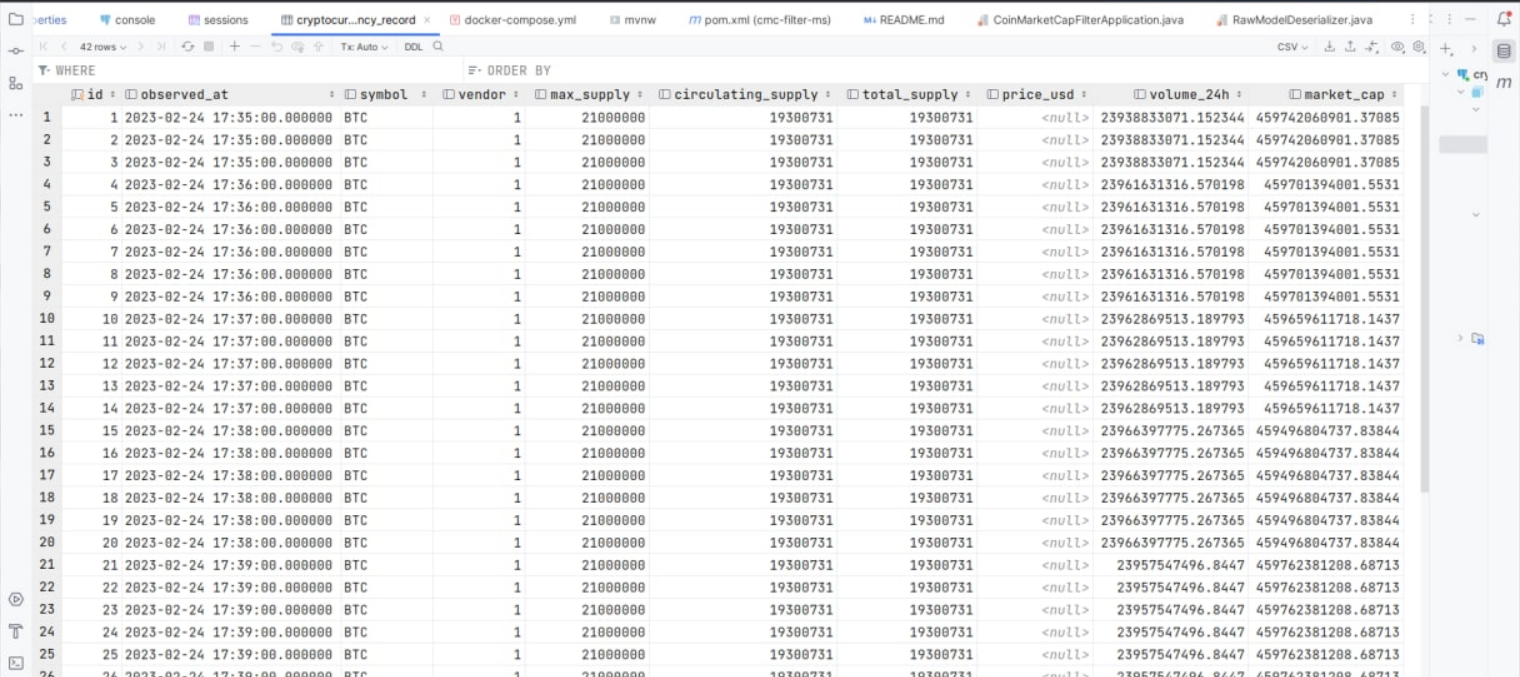
\includegraphics[width=1\columnwidth]{databasescreen.png}
    \caption{Изображение с содержанием базы данных }
\end{figure}

Также благодаря сбору метрик был реализован простой UI с помощью Prometheus и Grafana
для отображения системной информации о загруженности системы, а также графики
стоимости криптовалют за наблюдаемый промежуток.

\begin{landscape}
    \begin{figure}[!h]
        \centering
        % 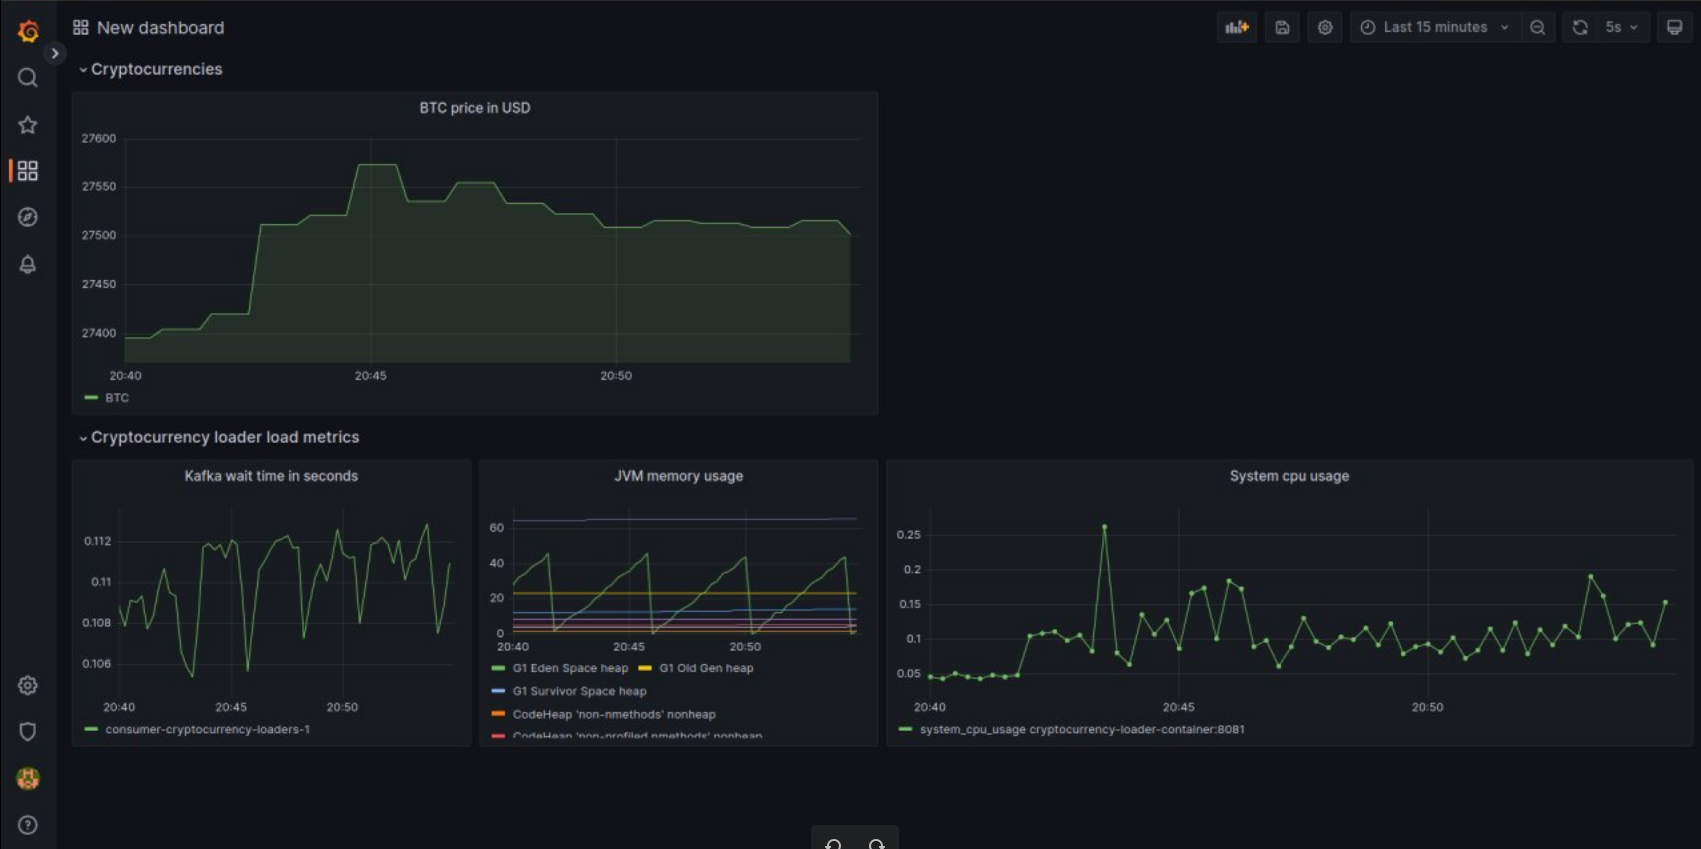
\includegraphics[width=1\columnwidth]{grafanascreen.png}
        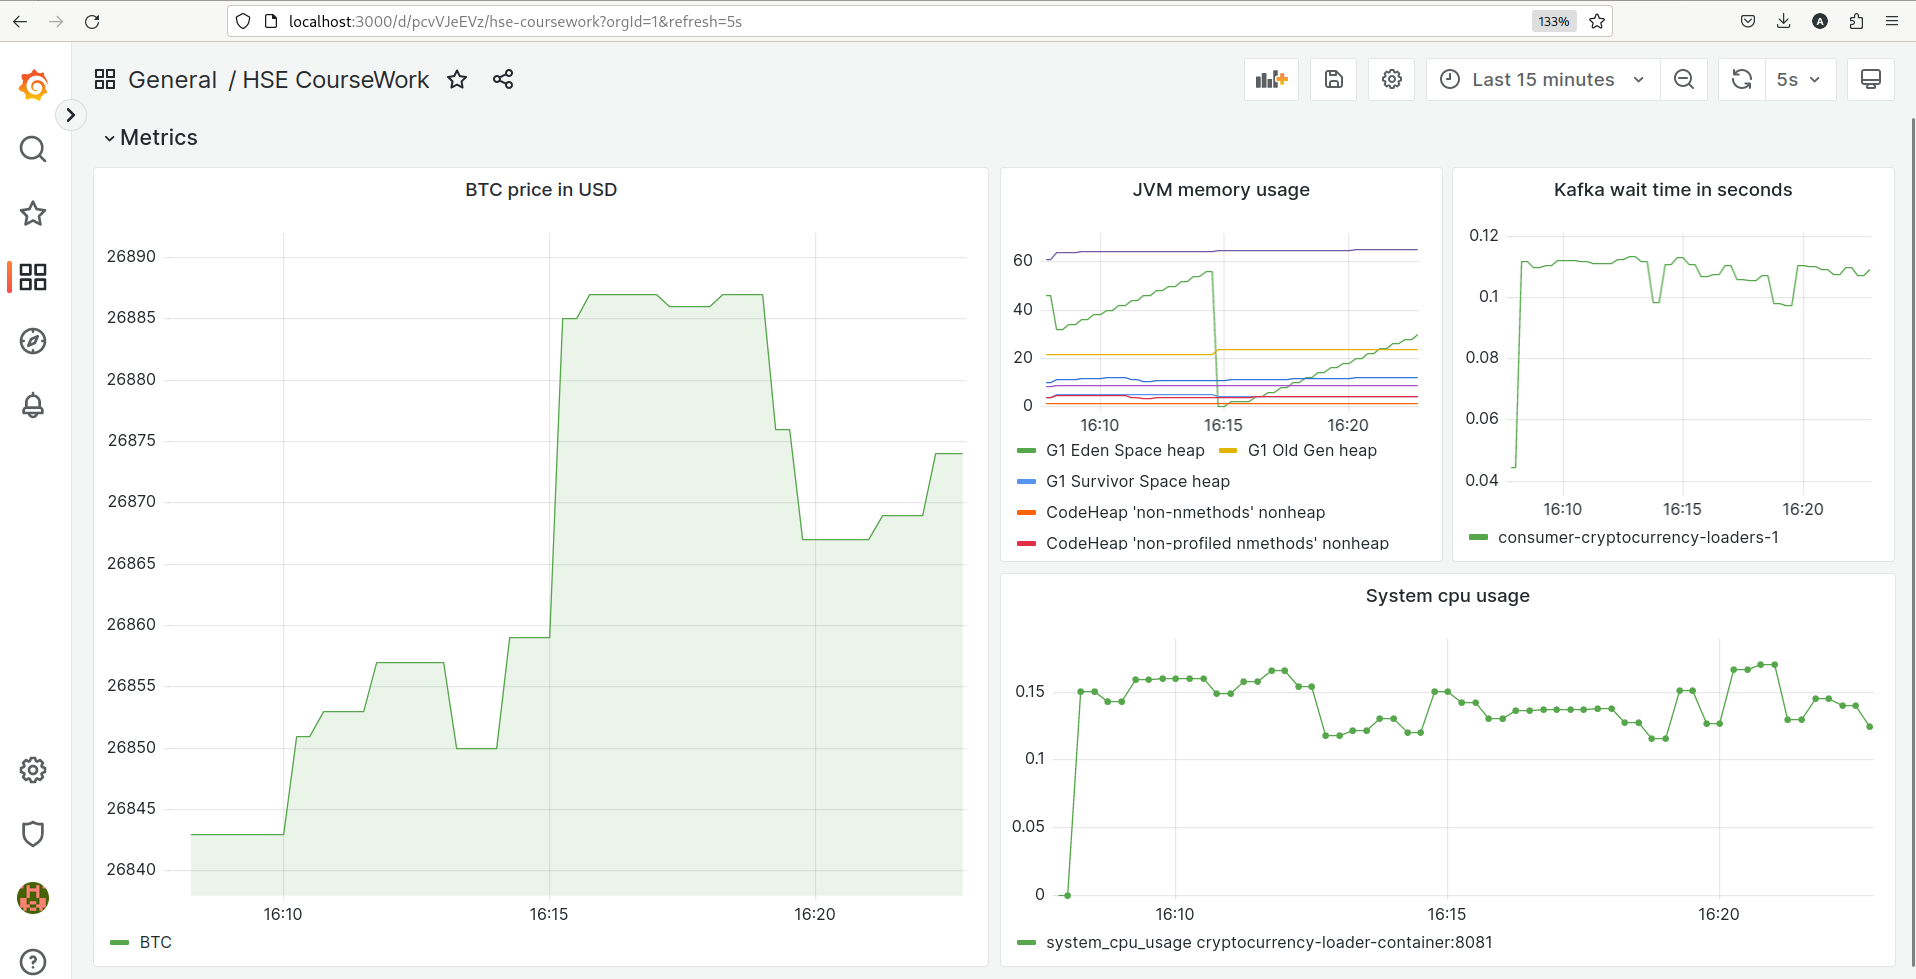
\includegraphics[height=0.8\textheight]{grafanav2.png}
        \caption{Изображение дашборда Grafana с графиком цены биткоина и системными метриками загруженности.}
        \label{grafana}
    \end{figure}
\end{landscape}

В целом система представляет собой мощный инструмент для обработки
real-time финансовых данных. Я использовал современные технологии и подходы,
чтобы обеспечить быстрый и надежный доступ к данным для наших пользователей. В
результате получилась высокоэффективная система, которая может быть
использована в различных областях финансовой деятельности.
